% !TEX encoding = UTF-8 Unicode
\documentclass[12pt,twoside]{report}
\usepackage[utf8]{inputenc}
\usepackage[T1]{fontenc}
\usepackage[francais]{babel, varioref}

\usepackage{afterpage}
\usepackage{calc}
\usepackage{color}
\usepackage{fancyhdr}
\usepackage{float}
\usepackage{graphicx}
\usepackage{helvet}
\usepackage{listings}
\usepackage{listingsutf8}
\usepackage{lscape}
\usepackage{textcomp}
\usepackage{xcolor}
\usepackage{xspace}
\usepackage[urlcolor=blue, linkcolor=black,linktoc=all, colorlinks=true]{hyperref}
\usepackage[left=2cm, right=2cm, top=2.1cm, bottom=2.5cm]{geometry}
\usepackage[final]{pdfpages}

\let\iint\undefined
\let\iiint\undefined

\begin{document}
\title{2D matrice pattern search}
\date{March 2018}
\maketitle

\clearpage

\setcounter{tocdepth}{4}
\setcounter{secnumdepth}{4}
\setcounter{page}{1}

\tableofcontents{}

%En cas d'ajout de .tex, copiez-collez cette ligne en modifiant le nom de fichier
% !TEX encoding = UTF-8 Unicode
\chapter{Backlogs}

\section{Project structure - 2h}
Implementation of solution code structure.

\begin{figure}[h]
    \begin{center}
        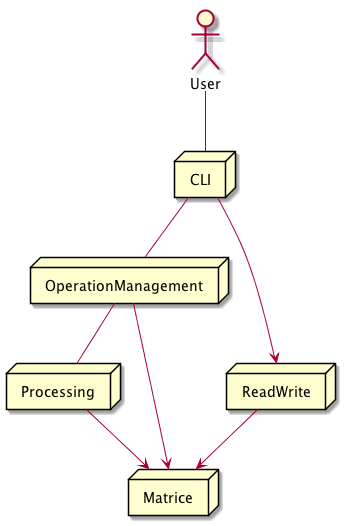
\includegraphics[scale=0.40]{./ressources/graph/deployment.png}
    \end{center}
    \caption{Deployment diagram}
    \label{Solution - Deployment diagram}
\end{figure}
\bigskip


\section{Command line interface - 1/2 day}
It should handle user entry in order to perform search.\\
It should process user entry to extract request information.\\
Assuming that the matrix data contains sensitive information, it should not be stored in plain text:\\
- Command line interface should handle system arguments specifying file path and encryption key.\\
- CLI should work with File processing class in order to work with specified file.\\
\begin{enumerate}
    \item user interface - 30m
    \item user entries processing - 2h30
    \item unit tests - 1h
\end{enumerate}

\section{Matrice structure - 1.5 day}
In order to optimise research, and to be able to perform several research on the same matrice,\\
we should store 2 dimensional matrix of integers from the plain text file into an optimal data structure.\\
Some time should be taken to review the different data structure possible, and responding to search criteria.\\
Algorithm will need to be implemented in order to perform 2D matrix from original file.\\
\begin{enumerate}
    \item Matrice data structure - 1/2d
    \item formating algorithm - 1/2d
    \item unit tests - matrice access, simple research - 1/2d
\end{enumerate}

\section{Operations management - 2 hours}
Handle pattern search request.\\
Manage list of operations to apply on specified 2D matrice.

\section{Search Features - 1.5 day}
There are 3 search functions to implement:
\begin{description}
    \item [search sequence] Find all rows that have a specific sequence of numbers (if that number sequence
appears more than once for that row, you only need to print it once)
    \item [search unordered] Find all rows that contain all of the required numbers (if number repeats, that row must
contain at least that many number)
    \item [search closest match] Find the row that has the closest match to a specific number sequence (just need to
consider the number of matches)
\end{description}
Search features should be of better complexity than O(n) (n is matrix element count).\\

\begin{enumerate}
    \item search management - 2h
    \item search algorithm - 1d
    \item units test - 1/2d
\end{enumerate}

\section{File Processor - 1 day}
User must be able to indicate the matrix data file they will be using through parameters(argc/argv).\\
File processor should be able to read the data from the plain text file into a simple data structure (array).\\
Assuming that the matrix data contains sensitive information, it should not be stored in plain text;\\
File processor should handle an encryption algorithm to hide/access sensitive information.\\
\begin{enumerate}
    \item read/write - 2h
    \item encryption - 1/2d
    \item file processing - 1h
    \item unit tests - 1h
\end{enumerate}

% !TEX encoding = UTF-8 Unicode
\chapter{Planning}

\section{Resumed Backlogs}
\begin{enumerate}
    \item Project structure - 2h
    \item Command line interface - 1/2d
    \item Matrice - 1.5d
    \item Operations management 2h
    \item Search features 1.5d
    \item FileProcessor 1d
\end{enumerate}

\section{Sprints}

Division into sprints of the development cycle.

\subsection{Sprint 1}
Sprint 1 should take 1.5 days.\\
This time will be used to review further the application organisation, and review algorithms to encrypt/unencrypt file.\\
It will contain the initialisation of the application code structure.\\
The implementation of reading and processing method for 2 dimensional matrix of integers representation file.\\
    \begin{itemize}
        \item 1 - Project structure
        \item 6 - File processor
    \end{itemize}

\subsection{Sprint 2}
Sprint 2 should take around 3.5 days.\\
This time will be used to review possibilities between pattern search algorithm, and data structure optimising research.\\
Implementation of an optimised Matrice data structure.\\
Implementation of 3 types research algorithms responding to requested features.\\
Testing of project criteria.
    \begin{itemize}
        \item 3 - Matrice
        \item 5 - Search features
    \end{itemize}

\subsection{Sprint 3}
Sprint 3 should take around 1.5 day.\\
It implies the implementation of the command line interface.\\
The implementation of search operations management used by CLI.\\
Testing and validation of full workflow.
    \begin{itemize}
        \item 2 - Command line interface
        \item 4 - Operations management
        \item Workflow validation
    \end{itemize}


% Liste des figures
\listoffigures

% Bibliographie

\nocite{*}
%\bibliography{tex/biblio}{}
%\bibliographystyle{plain}
%\printbibliography

% Annexes
\clearpage
\appendix
\input{tex/annexes.tex}

\end{document}
